The first claim Phase I establishes is that the minimally specified
substrate develops sensory-specific organization without any semantic
supervision. Three levels of evidence exist in the record, in increasing
order of specificity.

\subsection{Afferent organization}

Under repeated single-pattern training (40 presentations of pattern
\(A\)), the afferent weight vectors become sharply selective. At drive
end, the mean per-neuron mass is \(0.290\) for \(A\)-channel afferents
against \(0.026\) for the never-presented \(C\) channels (mean
selectivity \((A-C)/(A+C) = +0.906\), 49 of 52 neurons A-favoring).
Training on \(C\) produces the mirror image (\(-0.758\), 2 of 52
A-favoring). The two trained configurations are mutually distant
(full-matrix cosine 0.119; a leave-one-pair-out centroid decoder
recovers the training identity in 91\% of neurons) and stable across 20
seconds of post-drive silence (cosine to drive-end 0.986--0.993)
\cite{synmem}. Figure~\ref{fig:organization}(a) shows the per-neuron
afferent mass split for the A-trained run.

\subsection{Transient spike-pattern separation}

During the stimulus, the population's response is organized but the
pattern classes overlap. In E1's curriculum (patterns A/B/C interleaved,
360 presentations), within-pattern response profiles across S1 halves
correlate 0.97--0.99 --- stable assemblies --- while cross-pattern
profiles remain high (A\(\cdot\)B 0.79\(\rightarrow\)0.73,
A\(\cdot\)C 0.75\(\rightarrow\)0.70, B\(\cdot\)C 0.81\(\rightarrow\)0.81
early to late S1) \cite{e1proto}. Later separation attempts quantified
the plateau: mean late-S1 cross-pattern cosine 0.673 (E3) and 0.740
(E3b, with lateral inhibition), against a frozen 0.60 bar; median
selectivity 0.455 and 0.366 against a 0.50 bar
\cite{e3bproto}. Both dynamics interventions failed in the same
direction, which the records interpret as a representational (shared
recurrent pool, no inhibition-derived gating), not a rate-dynamics,
limit.

\subsection{Per-presentation count structure}

Under the CLLA-era curriculum the response is a per-presentation count
structure: 500 ms presentations of a learned pattern recruit nearly the
whole population with several thousand internal spikes (e.g.\ the
A-block presentations of the baseline blocked run fire 1{,}300--1{,}700
internal spikes each), collapsed to a 52-dimensional spike-count
vector. The count vector is the representation the readout instruments
use, and the one the information bottleneck dilutes
(§\ref{sec:bottleneck}); Figure~\ref{fig:organization}(b) shows the
per-presentation counts across the first block.

Taken together the records support:

\begin{quote}
\textbf{Demonstrated:} sensory-specific afferent structure emerges from
local STDP, budget normalization, and pruning without supervision;
per-presentation spike-count vectors are stimulus-locked and
repeatable.\\[1pt]
\textbf{Supported:} stable per-pattern assemblies exist, but their
cross-pattern separation is weak and resisted two dynamics
interventions (E3 adaptation, E3b inhibition).\\[1pt]
\textbf{Not established:} any claim about separation sufficient for
pattern decoding from population activity alone at a
scientifically useful threshold (the E3b bar failed).
\end{quote}

\begin{figure}[t]
\centering
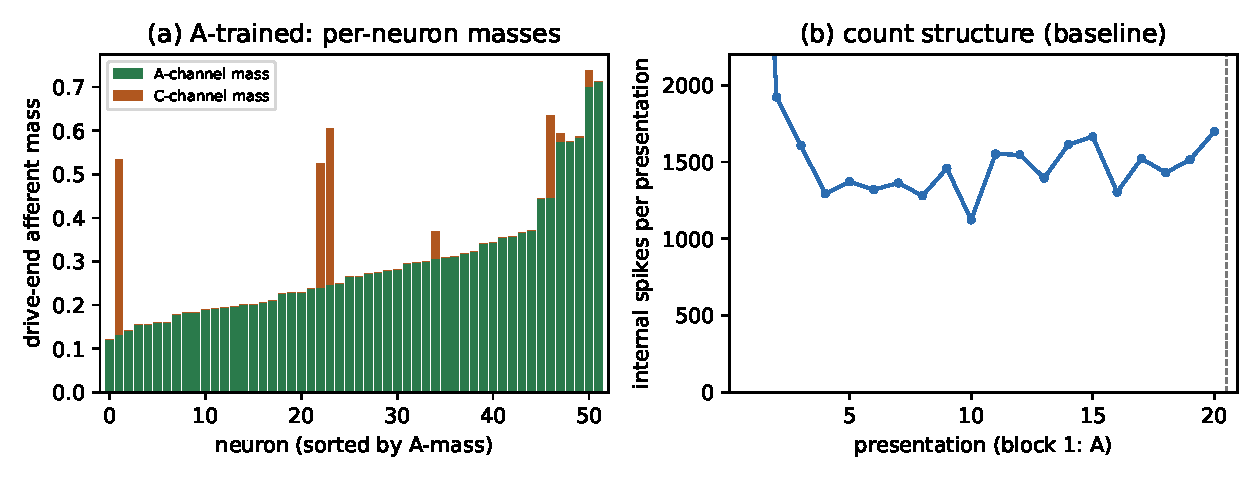
\includegraphics[width=\linewidth]{figures/fig2-organization.pdf}
\caption{\textbf{Emergent sensory organization}. (a) Drive-end
per-neuron afferent mass split (A-channel vs.\ C-channel) for the
A-trained single-pattern run; the population organizes along the
presented channel group (selectivity \(+0.906\), 49/52 neurons)
\cite{synmem}. (b) Per-presentation internal spike counts over the
first (A) block of the baseline blocked run --- the repeatable count
structure that subsequent regimes inherit. Data from preserved runs via
the committed instrument \texttt{rg8eval}.}
\label{fig:organization}
\end{figure}